%----------------------------------------------------------------------------------------
%
% LaTeX-template for degree projects at LNU, Department of Computer Science
% Last updated by Johan Hagelbäck, Oct 2015
% Linnaeus University
%
% License: Creative Commons BY
%
%----------------------------------------------------------------------------------------

%----------------------------------------------------------------------------------------
%	Settings and configuration
%----------------------------------------------------------------------------------------

\documentclass[a4paper,12pt]{article}
\usepackage[T1]{fontenc}
\usepackage{times}
\usepackage[english]{babel}
\usepackage[utf8]{inputenc}
\usepackage{caption}
\usepackage{subcaption}
\usepackage{wallpaper}
\usepackage[absolute]{textpos}
\usepackage[top=2cm, bottom=2.5cm, left=3cm, right=3cm]{geometry}
\usepackage{appendix}
\usepackage[nottoc]{tocbibind}
\usepackage[hidelinks]{hyperref}
\setcounter{figure}{0}
%\setcounter{secnumdepth}{3}
%\setcounter{tocdepth}{3}
\usepackage{amsmath}
\numberwithin{figure}{section}
\usepackage{sectsty}
\sectionfont{\fontsize{14}{15}\selectfont}
\subsectionfont{\fontsize{12}{15}\selectfont}
\subsubsectionfont{\fontsize{12}{15}\selectfont}

\usepackage{csquotes} % Used to handle citations

\renewcommand{\thetable}{\arabic{section}.\arabic{table}}  
\renewcommand{\thefigure}{\arabic{section}.\arabic{figure}} 

%----------------------------------------------------------------------------------------
%	
%----------------------------------------------------------------------------------------
\newsavebox{\mybox}
\newlength{\mydepth}
\newlength{\myheight}

\newenvironment{sidebar}%
{\begin{lrbox}{\mybox}\begin{minipage}{\textwidth}}%
{\end{minipage}\end{lrbox}%
 \settodepth{\mydepth}{\usebox{\mybox}}%
 \settoheight{\myheight}{\usebox{\mybox}}%
 \addtolength{\myheight}{\mydepth}%
 \noindent\makebox[0pt]{\hspace{-20pt}\rule[-\mydepth]{1pt}{\myheight}}%
 \usebox{\mybox}}

%----------------------------------------------------------------------------------------
%	Title section
%----------------------------------------------------------------------------------------
\newcommand\BackgroundPic{
    \put(-2,-3){
    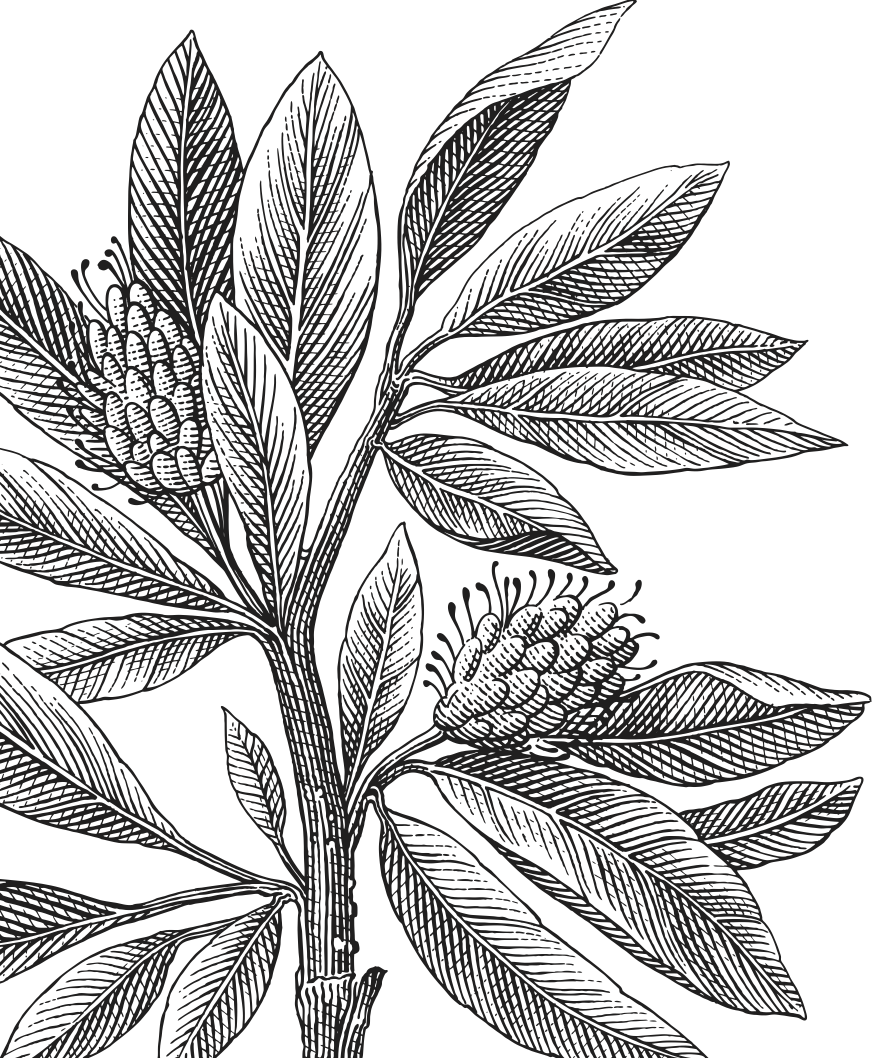
\includegraphics[keepaspectratio,scale=0.3]{img/lnu_etch.png} % Background picture
    }
}
\newcommand\BackgroundPicLogo{
    \put(30,740){
    
\includegraphics[keepaspectratio,scale=0.10]{img/logo.png} % Logo in upper left corner
    }
}

\title{	
\vspace{-8cm}
\begin{sidebar}
    \vspace{10cm}
    \normalfont \normalsize
    %\Huge Bachelor/Master Thesis Project \\
    \vspace{-1.3cm}
\end{sidebar}
\vspace{3cm}
\begin{flushleft}
    \huge Computer networks - 1DV701 \\ 
    \LARGE  Assignment 3\\
\end{flushleft}
\null
\vfill
\begin{textblock}{6}(10,13)
\begin{flushright}
\begin{minipage}{\textwidth}
\begin{flushleft} \large
\emph{Author:} Michael Johansson \& Jakob Heyder\\ % Author
%\emph{Supervisor:} Name of your supervisor\\ % Supervisor
%\emph{Examiner:} Dr.~Mark \textsc{Brown}\\ % Examiner (course manager)
\emph{Semester:} VT 2017\\ % 
%\emph{Subject:} Computer Science\\ % Subject area
\end{flushleft}
\end{minipage}
\end{flushright}
\end{textblock}
}

\date{} 

\begin{document}
\pagenumbering{gobble}
\newgeometry{left=5cm}
\maketitle
\clearpage


%----------------------------------------------------------------------------------------
\newpage
\pagenumbering{gobble}
\tableofcontents % Table of contents
\newpage
\pagenumbering{arabic}

%----------------------------------------------------------------------------------------
%
%	Here follows the actual text contents of the report.
%
%----------------------------------------------------------------------------------------

\section{Assignment summary}

\begin{itemize}
\item\textbf{Michael}
Work percentage 50\%

\item\textbf{Jakob} 
Work percentage 50\%
\end{itemize}



\newpage

\section{Problem one}

In figure \ref{TFTP_READ} we show a successful RRQ (Read-Request) to the implemented tftp server retrieving a small test-text file.
\newline \noindent
We use the original socket as a kind of server socket accepting the requests on port 4970 (Usually 69 in TFTP) and then after receiving a request, either write or read, we open a new thread for the specific client connection. In this thread we use the sending socket which acquires a free port (zero port indicates to get a random free port e.g. 5800) and then send the new specified port to the client in the ACK (WRQ) or DATA (RRQ) packet.  This is defined in the TFTP-Specification that the initialization will be on a predefined port and then the server communicates the used port to the client. This way we can also handle multiple client requests since the original socket is freed after handling the client in a separate thread. Also the send socket connects to the remote port and address of the client given from the request.

\begin{figure}[h!]
	\centering
	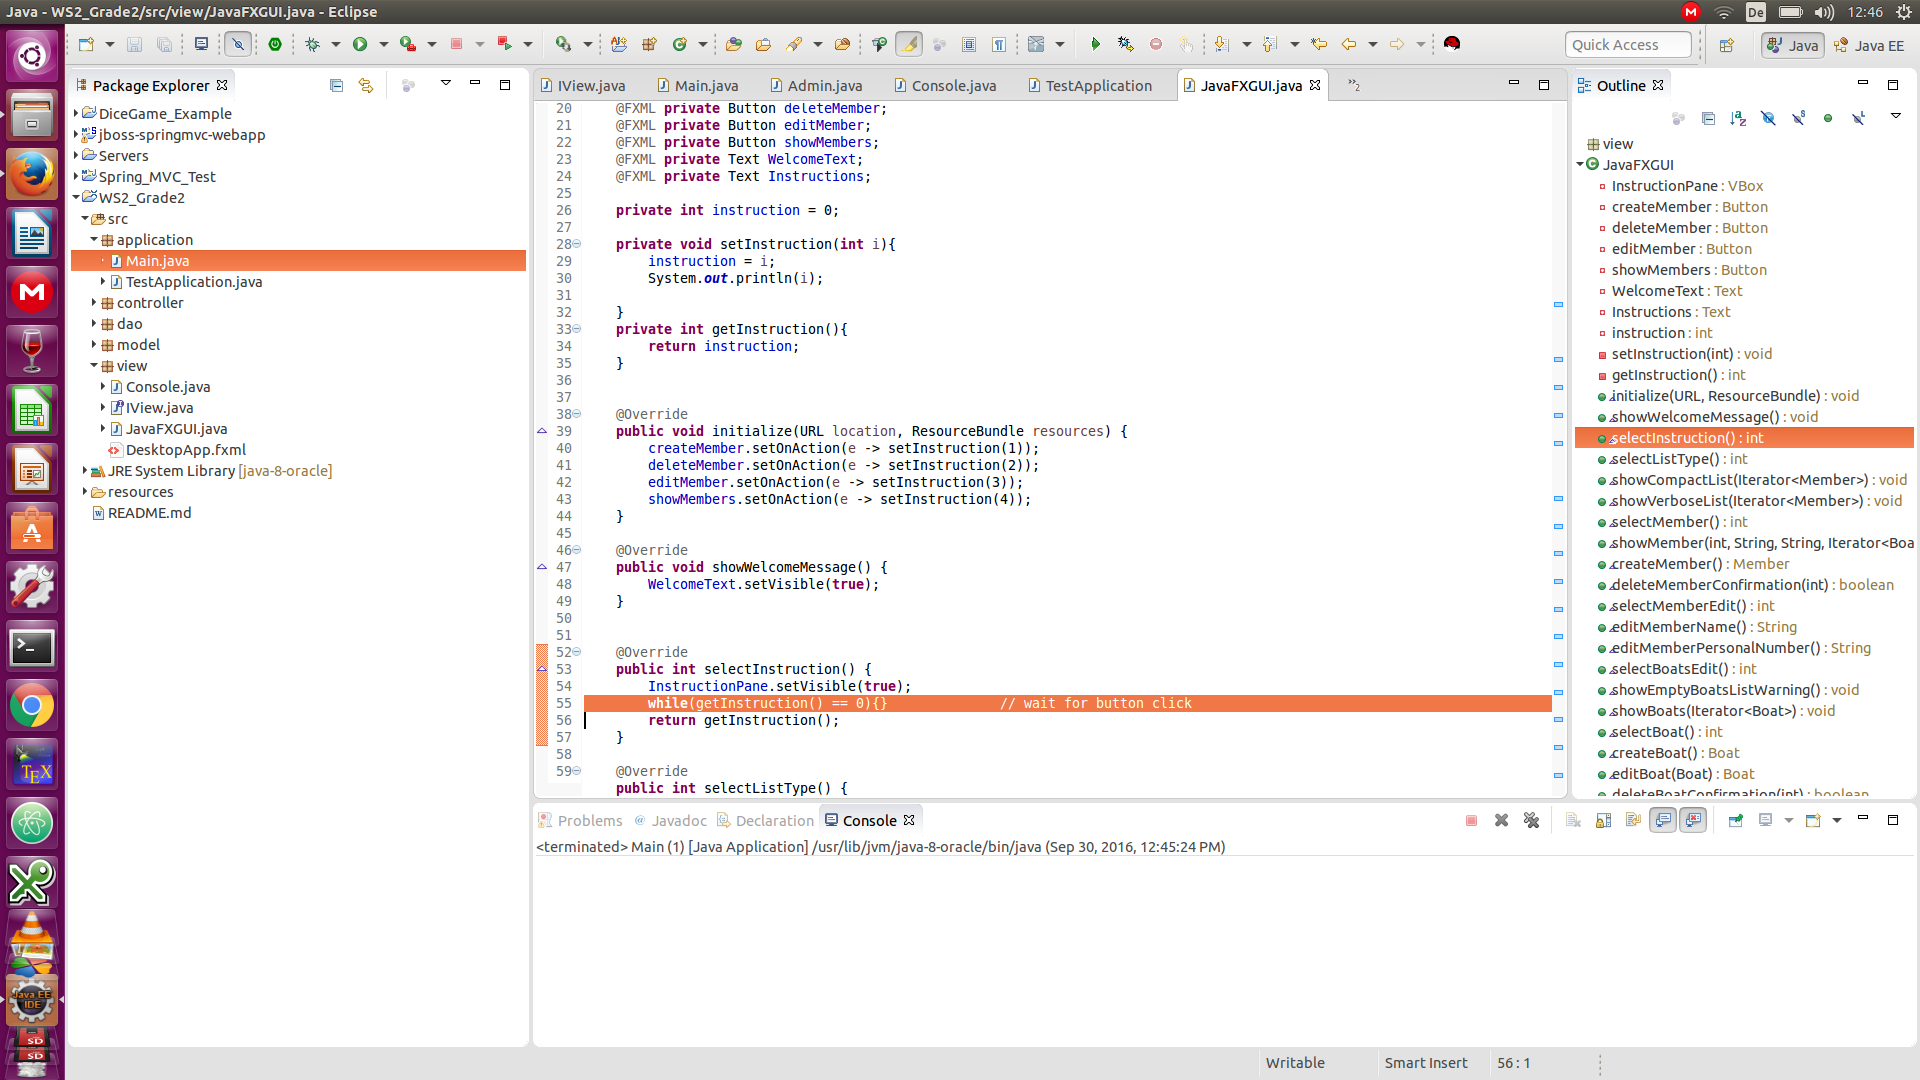
\includegraphics[width=0.95\textwidth,keepaspectratio]{img/problem1.png} 
	\caption{Successful READ-Request. We can see the tftp-client in the terminal window, eclipse tftp server and the home directory where the retrieved file is saved to.}
	\label{TFTP_READ}
\end{figure}

 

\newpage
\section{Problem two}

In figure \ref{TFTP_READ_WRITE} we send and receive multiple large files. The task says sending but it is not clear if it means sends from client or server. However both is on the screenshot with files larger then 512 bytes. The case of files which are so large that they exceed the package number of a short is thought of but not mentioned in the specification. Therefore its left out and assumed out of scope in this assignment. 
\newline \noindent
We implemented a timeout mechanism that the sending socket times out if it does not receive the next DATA/ACK packet in 150ms. If it times out it will try to retransmit or simply tries to receive again. We have a retransmission counter which will be increased and stops the execution after 5 retransmissions/waiting-times so that no infinite loop will occur. 

The execution of a write-request can be seen also on figure \ref{TFTP_READ_WRITE}. 

\begin{figure}[h!]
	\centering
	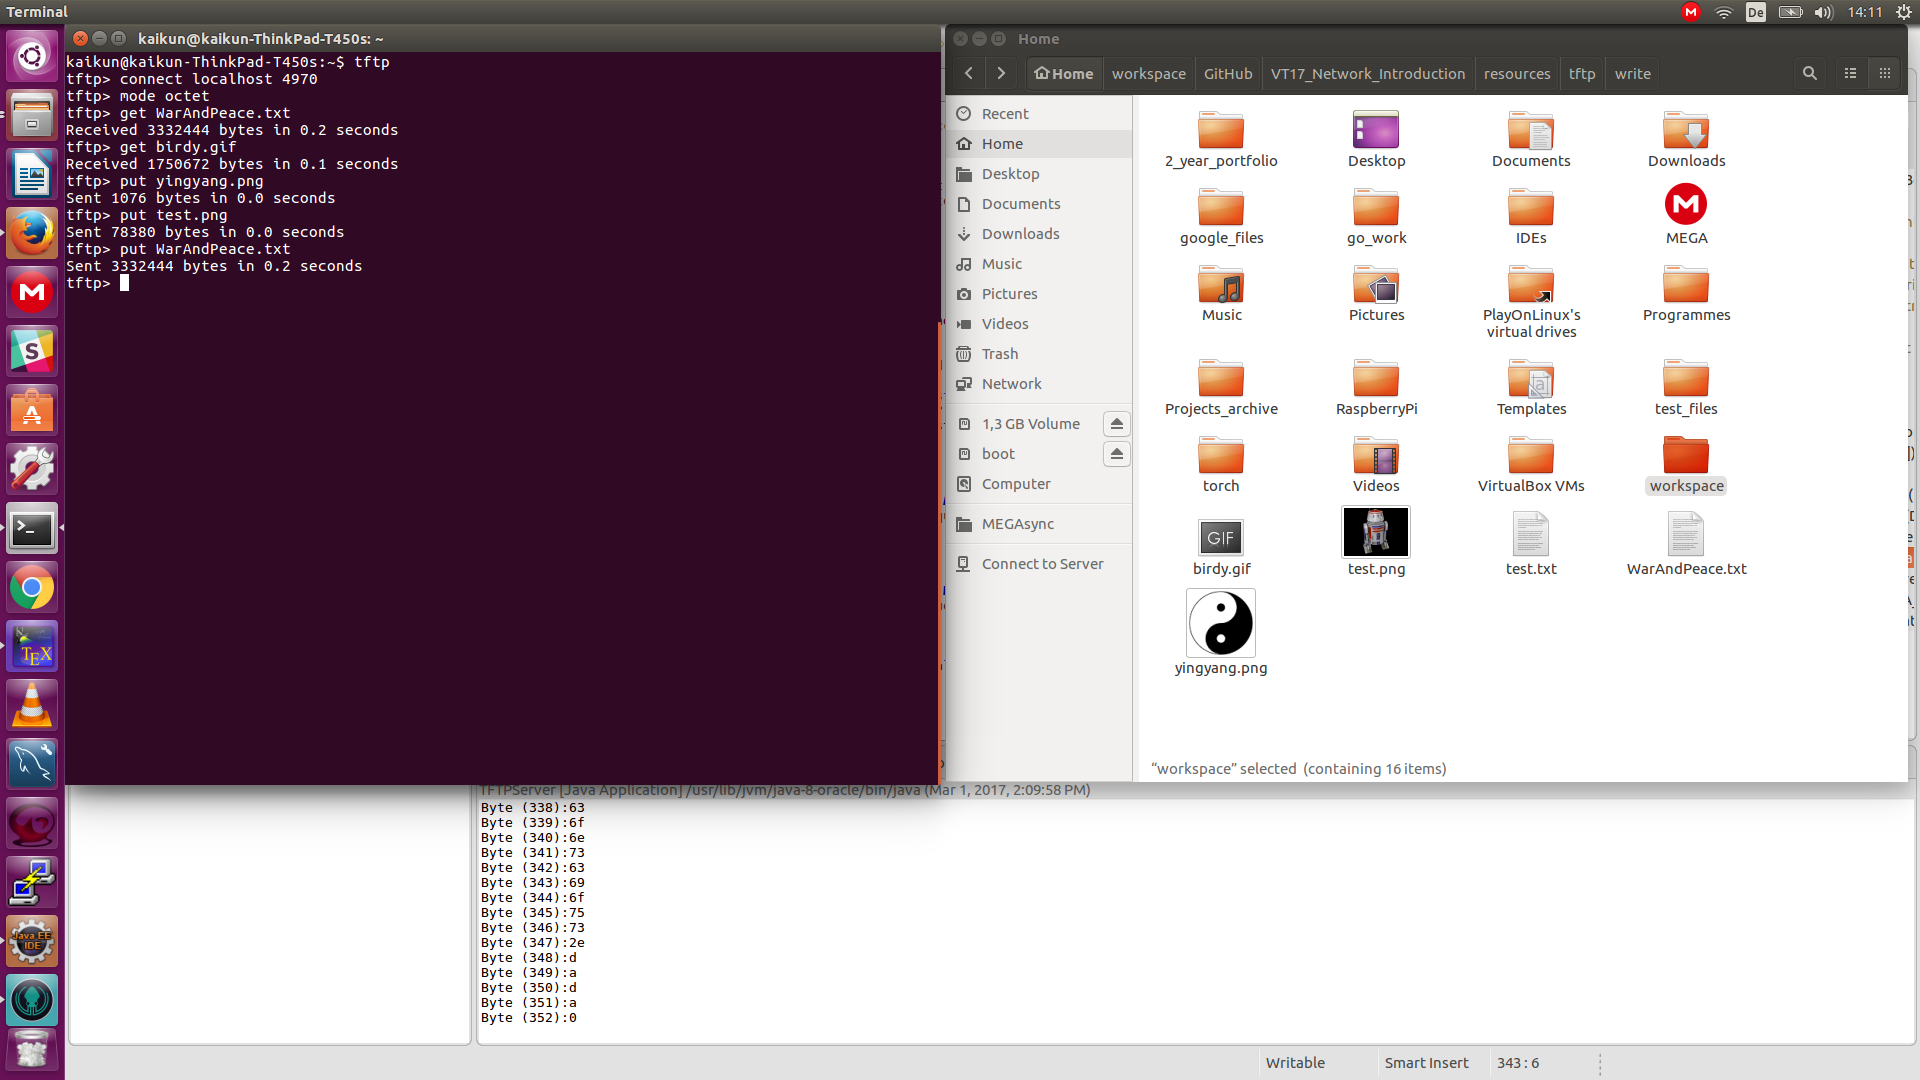
\includegraphics[width=0.95\textwidth,keepaspectratio]{img/ReadWriteMultipleFiles.png} 
	\caption{Read and write multiple large files. On the left hand side we see the tftp client transfering files from the home directory or reading files from the server. We can see the bytes transfered.}
	\label{TFTP_READ_WRITE}
\end{figure}

\newpage
\subsection{VG.1 wireshark analyze}

In figure \ref{ws1} we can see the line marked where the client, in this case with the localhost - 127.0.0.1 - src-address from the randomly choosen free port 53874 is sending a UDP Packet to the server. The server address is also localhost - 127.0.0.1 - dest-address and the port is the chosen 4970, which is usually 69 for the TFTP protocols. In the bottom rows we can see the content of the package and beside all the headers of the lower layers the data of the UDP packet is marked. In the data we can see it start with the 2Bytes 00 01 which is defined in the TFTP-Specification as the operational code for a read request. The next bytes, in this case 8, until a zero byte are defined as the filename string. After the zero byte the mode will be defined by the following bytes closed with a zero byte again. In this case we can see that the OP-Code is RRQ, the filename of the requested file is test.txt and the mode is octet.
\newline \noindent
\newline \noindent
In figure \ref{ws2} we can see the line marked where the server answers to the clients read request. We see that the destination and source address are again localhost, but would have switched. The switch we can identify on the ports, while the client port 53874 is now the receiving port the sending port from the server changed to 53964. This tells the client that this will be the port on the server side used for the rest of the file transmission. The initial port 4970 is only used to handle new requests. In the bottom rows we can see the data send back from the server. It starts with the 2Bytes 00 03 which is the OP-Code for DATA packages recording to the TFTP-Specification. The next two bytes 00 01 indicate the package number. In this case it is the first data package sent. It follows the actual file-data. In this case it is a text file and simply transfers the ASCII-Characters saved in it, "This is a test.".
\newline \noindent
\newline \noindent
In figure \ref{ws3} we can see the line marked where the client sends an acknowledgement back to the server that it received the data package. We can see that the source and destination port flipped again and that the client now sends to the server port it received the data package from. The client sends only 4 Bytes data back. The first two indicating the OP-Code again in this case 00 04, meaning it is an acknowledgment packet and 2 more bytes 00 01 referencing the package number of the received packet which gets acknowledged. Due to the fact that the received data package was less than 516 bytes (512 inc. 4bytes header data) the client knows that the file is complete and with sending the ACK-Packet back the connection is terminated normally.

\begin{figure}[h!]
	\centering
	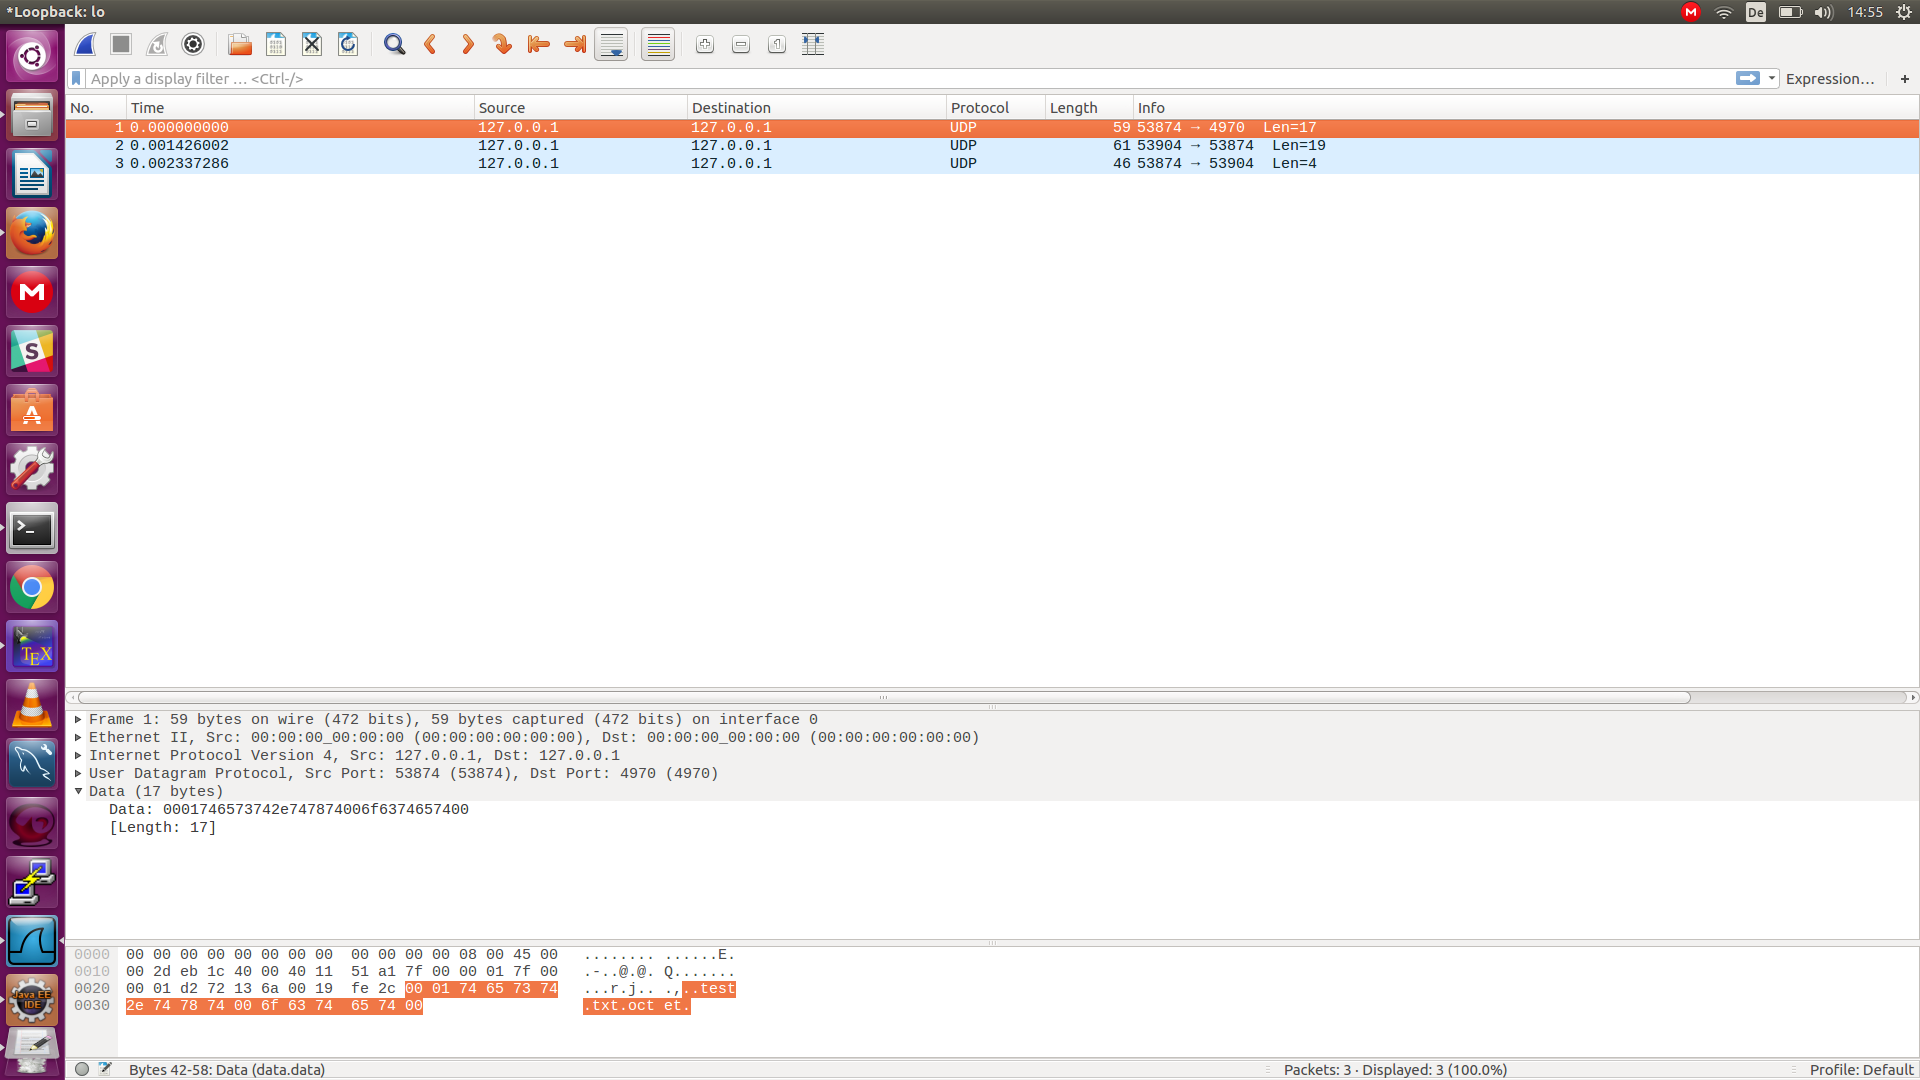
\includegraphics[width=0.95\textwidth,keepaspectratio]{img/Line1Wireshark.png} 
	\caption{We see a screen of a read request in wireshark. The send data, which is a TFTP-RRQ is marked in the bottom rows.}
	\label{ws1}
\end{figure}

\begin{figure}[h!]
	\centering
	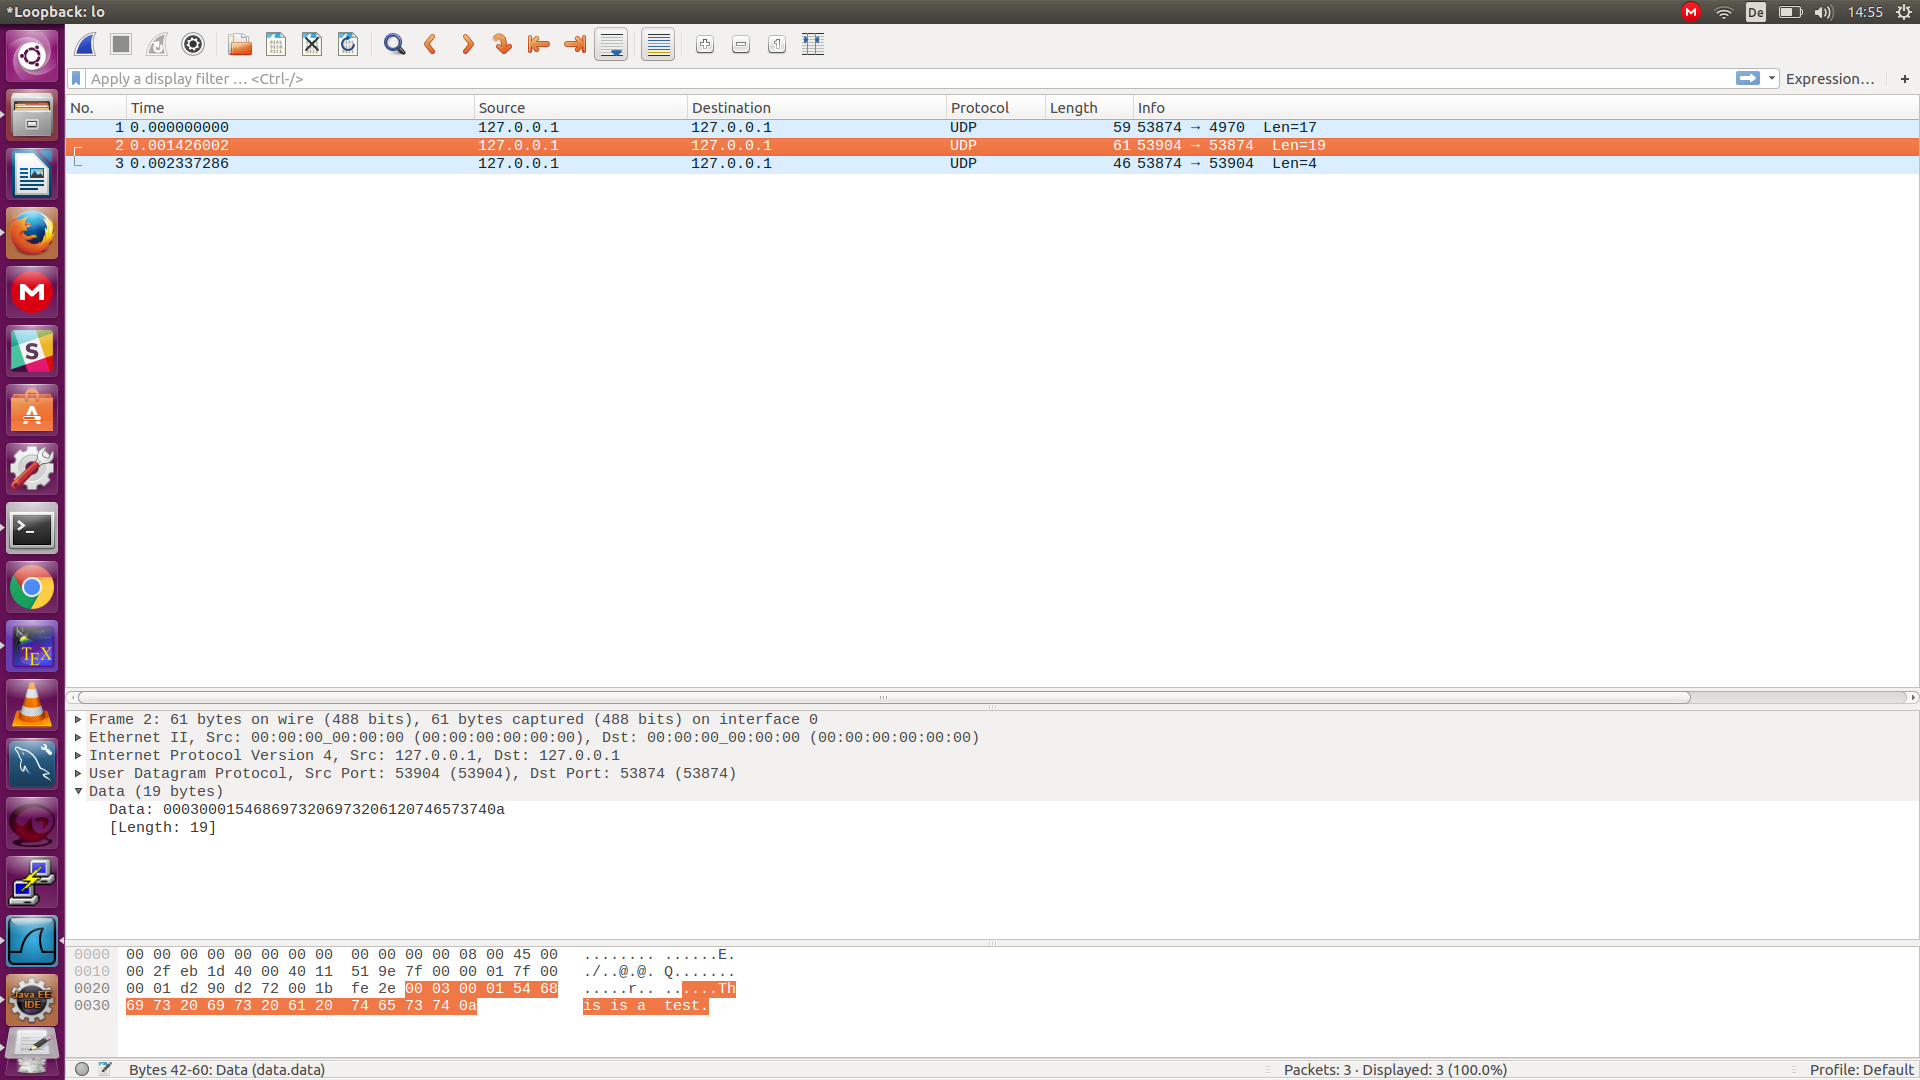
\includegraphics[width=0.95\textwidth,keepaspectratio]{img/Line2Wireshark.png} 
	\caption{We see a screen of the answer from the TFTP-server to TFTP-RRQ in wireshark. The send data, which includes the file-data inc. TFTP-Header (DATA-OPCODE and packet number) is marked in the bottom rows.}
	\label{ws2}
\end{figure}

\begin{figure}[h!]
	\centering
	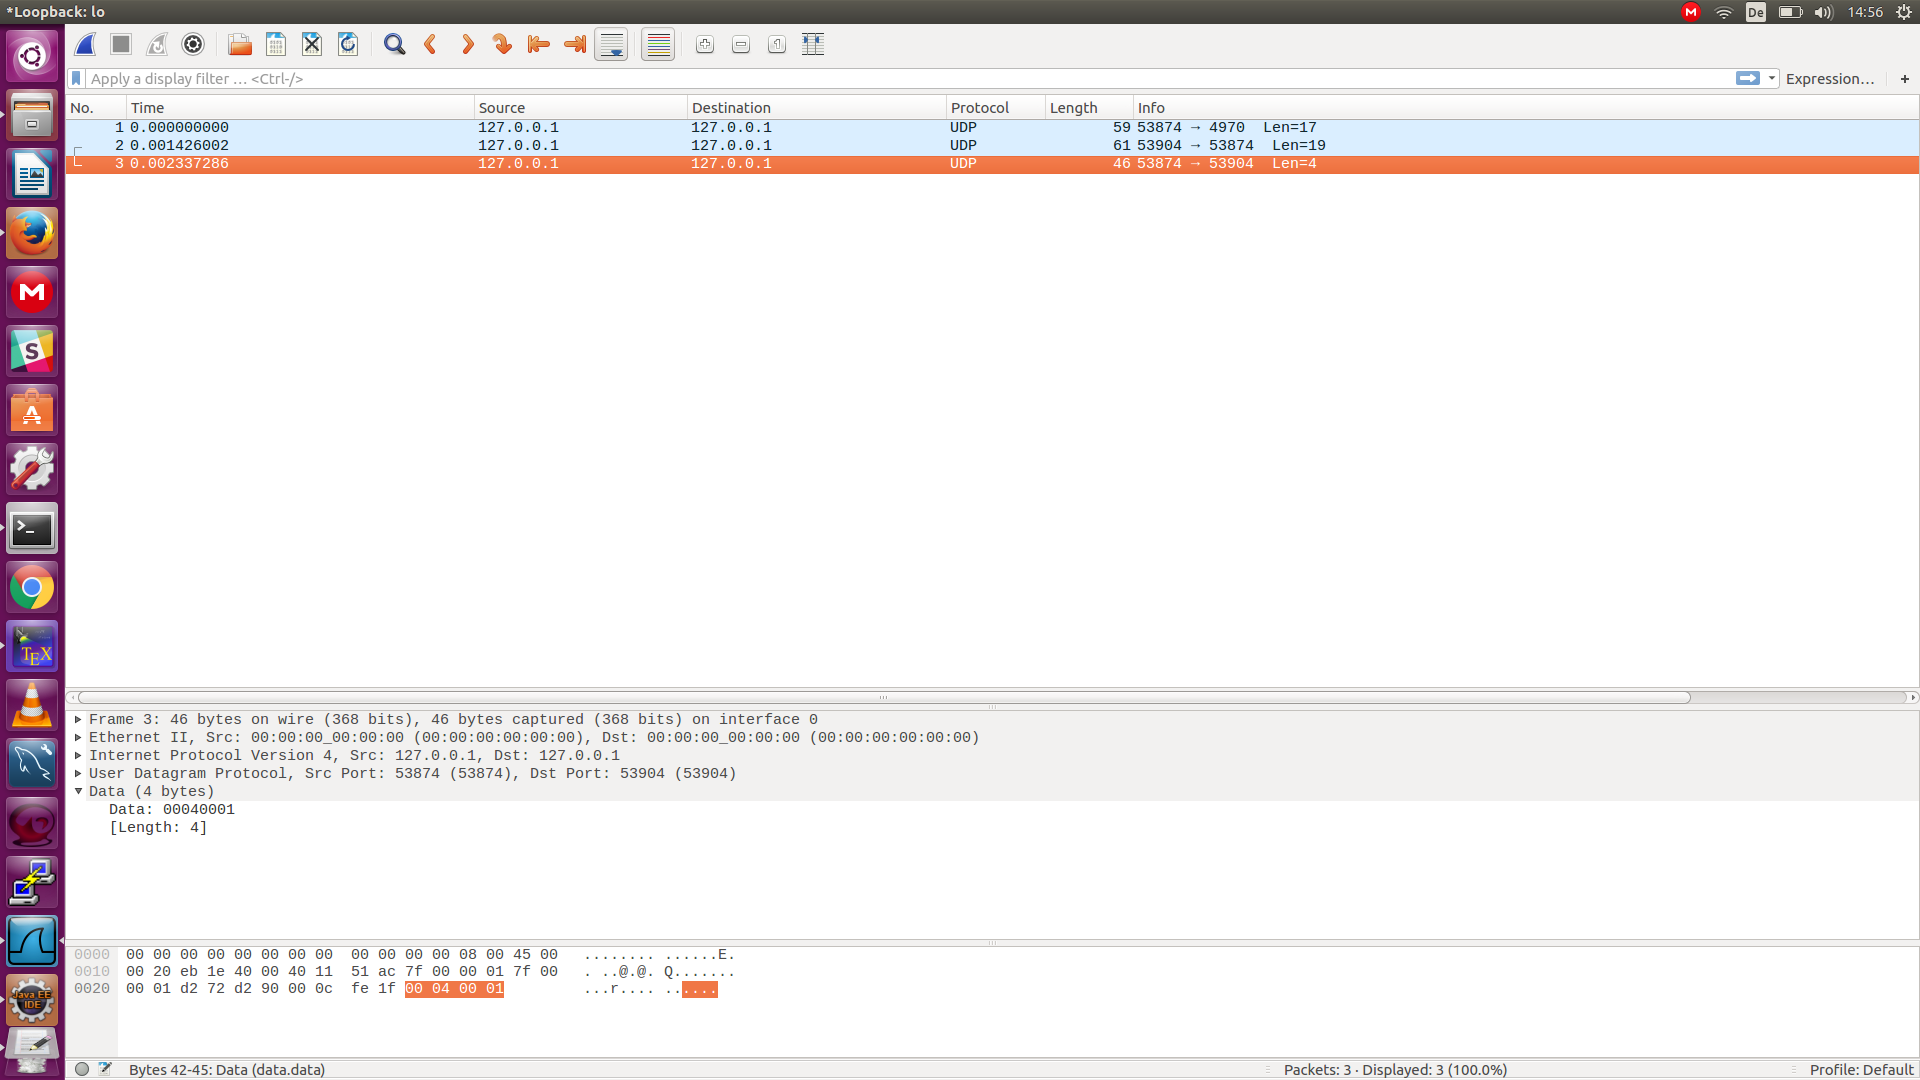
\includegraphics[width=0.95\textwidth,keepaspectratio]{img/Line3Wireshark.png} 
	\caption{We see a screen of the acknowledgement of the TFTP-client to the received data file of the TFTP-Server. The data is again marked in the bottom rows.}
	\label{ws3}
\end{figure}

\newpage

\section{Problem three}

In the figure \ref{error 0} we can se how our server sends an error packet for when the connection times out. The first two bytes is 05 to show that is an error packet. 
\begin{figure}[h!]
	\centering
	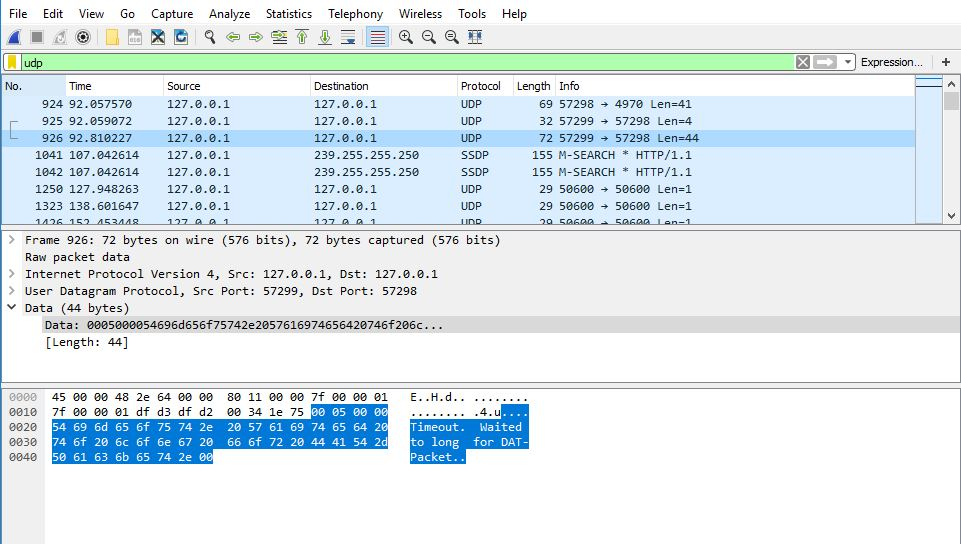
\includegraphics[width=0.95\textwidth,keepaspectratio]{img/error0.jpg} 
	\caption{}
	\label{error 0}
\end{figure}

\begin{figure}[h!]
	\centering
	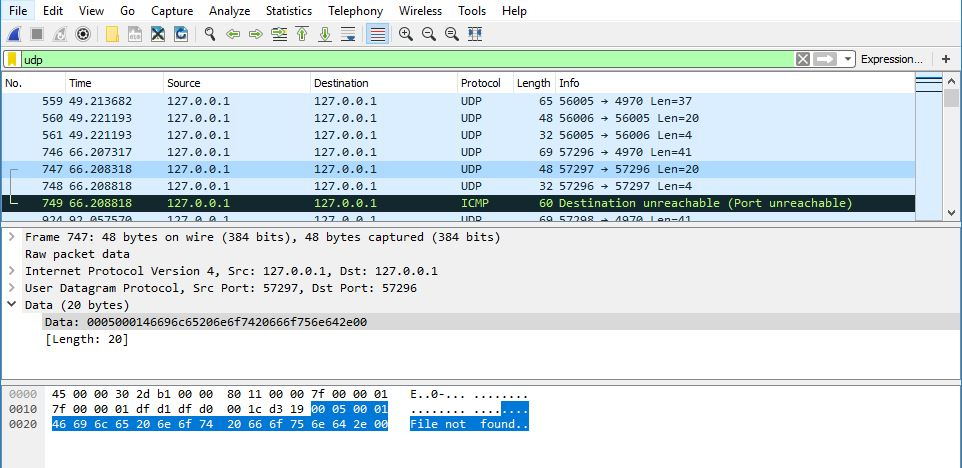
\includegraphics[width=0.95\textwidth,keepaspectratio]{img/error1.jpg} 
	\caption{}
	\label{error 1}
\end{figure}

\begin{figure}[h!]
	\centering
	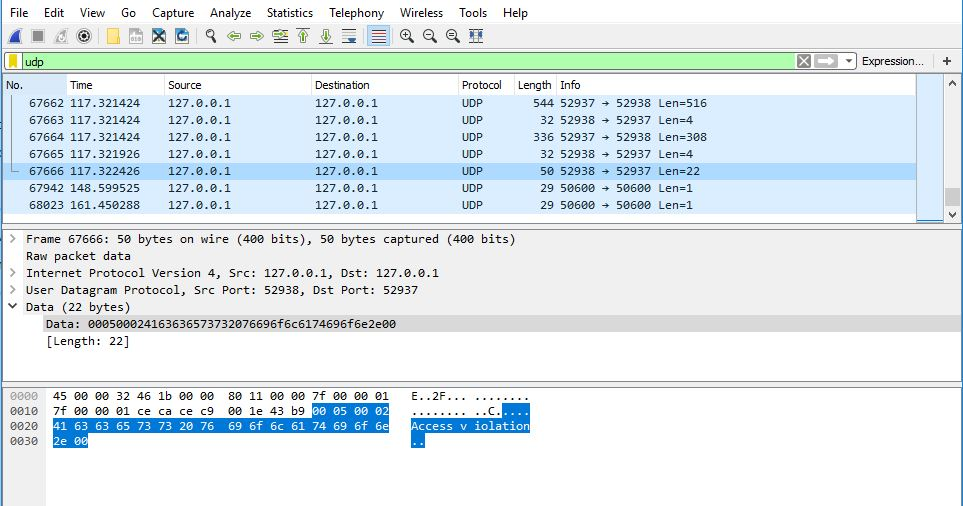
\includegraphics[width=0.95\textwidth,keepaspectratio]{img/error2.jpg} 
	\caption{}
	\label{error 2}
\end{figure}

\begin{figure}[h!]
	\centering
	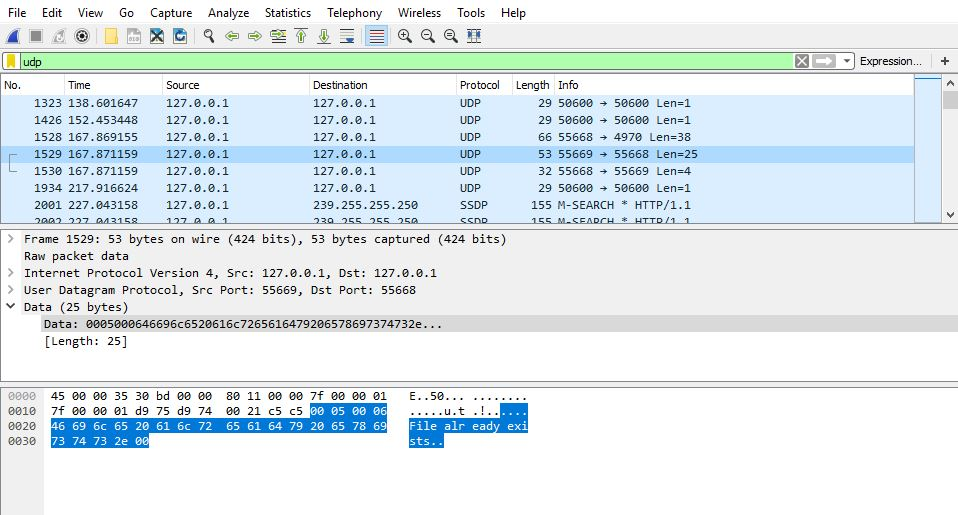
\includegraphics[width=0.95\textwidth,keepaspectratio]{img/error6.jpg} 
	\caption{}
	\label{error 6}
\end{figure}

\newpage

\subsection{VG.2 Remaining error codes}

\begin{figure}[h!]
	\centering
	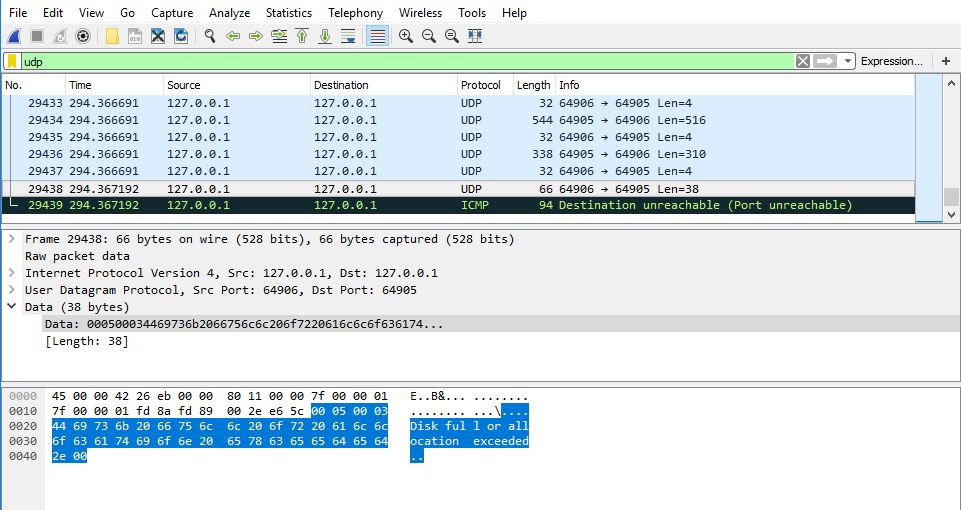
\includegraphics[width=0.95\textwidth,keepaspectratio]{img/error3.jpg} 
	\caption{}
	\label{error 3}
\end{figure}

\begin{figure}[h!]
	\centering
	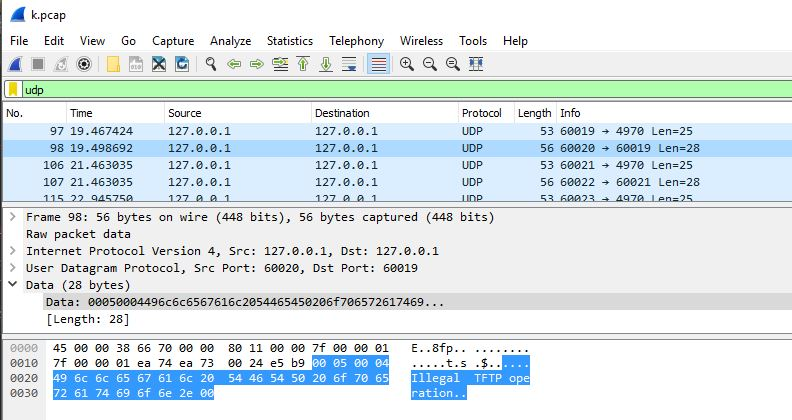
\includegraphics[width=0.95\textwidth,keepaspectratio]{img/error4.jpg} 
	\caption{}
	\label{error 4}
\end{figure}

\begin{figure}[h!]
	\centering
	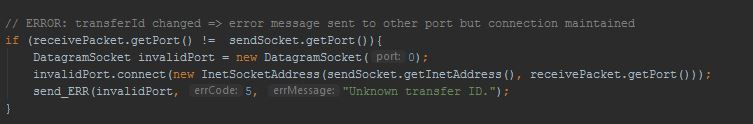
\includegraphics[width=0.95\textwidth,keepaspectratio]{img/error5.jpg} 
	\caption{}
	\label{error 5}
\end{figure}

\end{document}
